In 2012 AlexNet~\cite{krizhevsky2012imagenet} won on ILSVRC2012 classification task by a large margin compared to the non deep learning algorithms. The goal of this classification challenge is to train a model that classifies an input into 1,000 categories. Models are trained on a very large dataset containing 1.2 million images, with 50,000 images for validation, and 100,000 for test set. The training set is derived from the ImageNet~\cite{deng2009imagenet} project that contains images from almost 22,000 categories. The AlexNet contains 5 convolutional layers and 3 fully connected layers as depicted in Figure~\ref{fig:Alex_net}.

According to the universal approximation theory~\cite{hornik1989multilayer} a feed-forward network is able to approximate any measurable function to any desired degree of accuracy. However the layer can become very wide that is good at memorization prone to overfitting the data and not so good at generalization to new unseen data. Therefore, the trend after AlexNet was to increase the number of layers, so as to create deeper networks that are able to generalize better on unseen data. As a result of this tendency new architectures have been presented that achieved state-of-the-art performance on the contest and are going to be discussed to the following sections.

\begin{figure}[]
    \begin{center}
    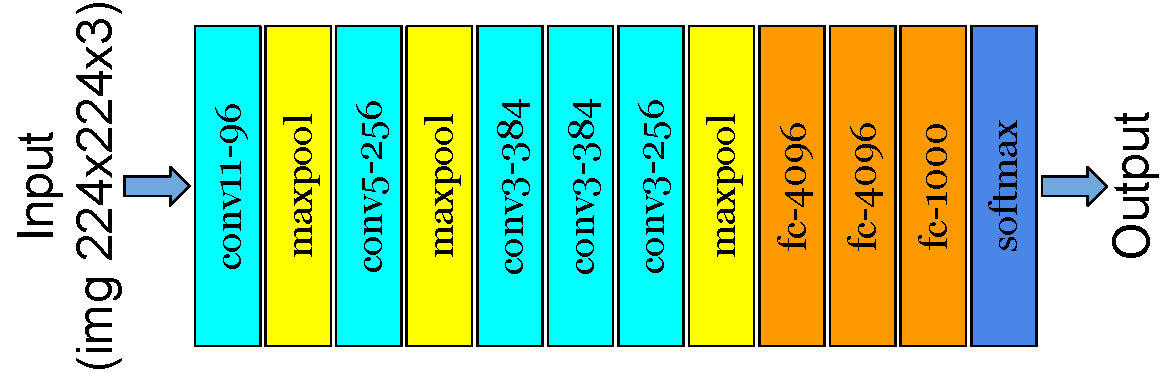
\includegraphics[width=0.6\textwidth]{images/Alex_net.pdf}
    \end{center}
    \caption{AlexNet architecture} \label{fig:Alex_net}
\end{figure}

\section{VGG}

The VGG architecture was introduced by the VGG group at Oxford University in 2014~\cite{simonyan2014very}. It simply replaces the large kernel filters from AlexNet from the first two convolutional layers with $3 \times 3$ kernel filters stacked on top of each other in increasing depth. The basic idea is that multiple smaller kernels are better than the one with larger kernel because multiple small sized kernels increase the depth of the network and as a result it can learn more complex features. Max pooling layers are used between the convolutional layers that reduce the number of network's parameters. The convolutional layers are followed by two fully connected layers each with 4,096 nodes, then by one fully connected layer with 1,000 nodes and finally by the softmax layer that assigns probabilities to the classes. So they introduced two versions of VGG network, one with 16 layers called VGG16 presented at Figure~\ref{fig:VGG16_imagenet}, and a deeper architecture with 19 layers. VGG network first introduced the idea that networks have to have a deep structure in order to extract complex features as you go deeper. 

\begin{figure}[]
    \begin{center}
    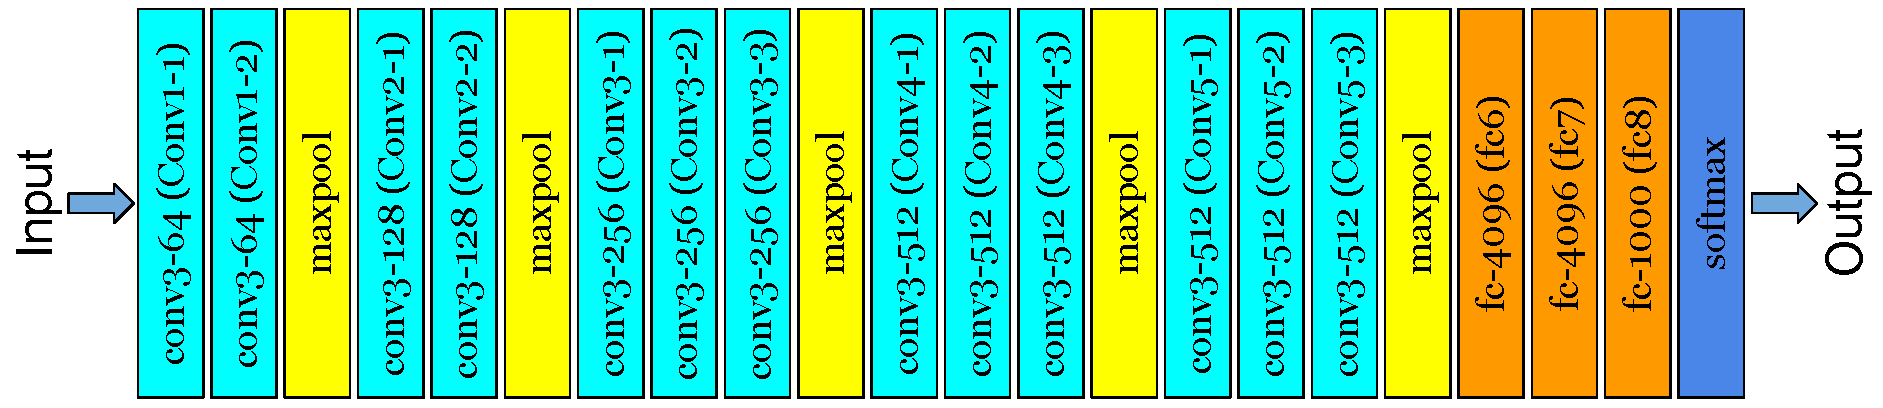
\includegraphics[width=0.8\textwidth]{images/VGG16_imagenet.pdf}
    \end{center}
    \caption{VGG16 architecture} \label{fig:VGG16_imagenet}
\end{figure}


\section{GoogLeNet/Inception}
Besides the fact that VGG architecture achieved state-of-the-art results on ImageNet dataset, stacking all these layers and all these number of filters has a huge computational and memory cost. The GoogLeNet architecture~\cite{szegedy2015going} builds on the idea that most of the activations in a deep network are either zero or unnecessary because of correlations between them. GoogLeNet is a 22 layer CNN that firstly escaped from the idea that deep networks had to be built by simply stacking convolutional layers, pooling layers, and fully connected layers in a sequential structure. So they introduced the "inception" micro-architecture depicted in Figure~\ref{fig:GoogLeNet}. The "inception" module acts on the same input with different convolutional filters and does pooling at the same time. All results are then concatenated before being fed to the next layer of the network. This allows the model to extract features of different sizes. 

\begin{figure}[]
    \begin{center}
    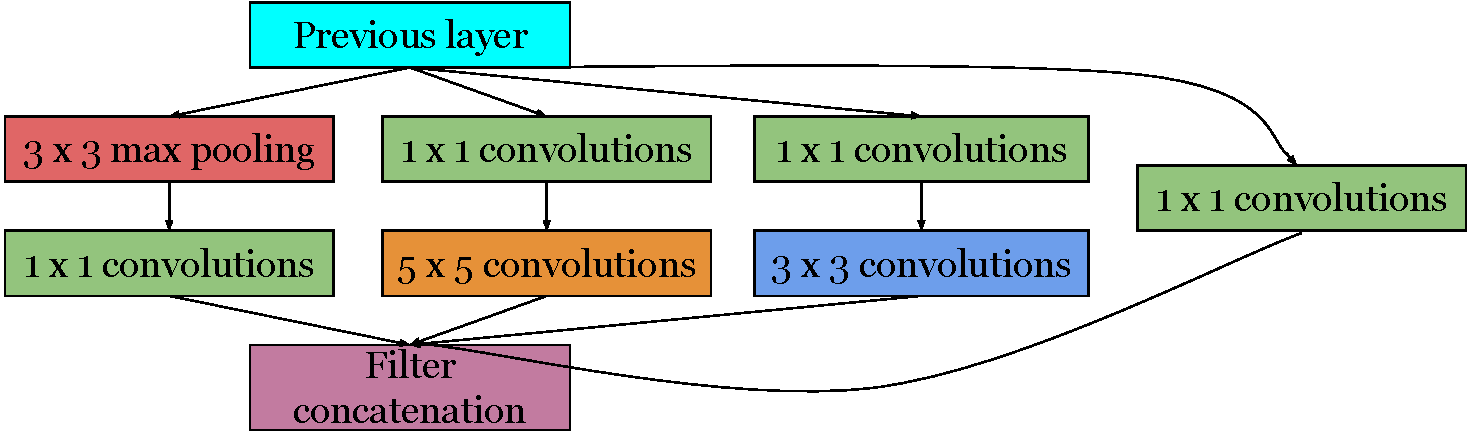
\includegraphics[width=0.8\textwidth]{images/GoogLeNet.pdf}
    \end{center}
    \caption{The inception module used in GoogLeNet.} \label{fig:GoogLeNet}
\end{figure}


\section{Residual Networks}
Residual networks were born from the simple observation that very deep networks perform worse from their shallower counterparts, that is, the performance with the addition of many layers saturates or even degrades rapidly. This observation is counter-intuitive since we could stack layers with identity mappings on the network and the resulting architecture should perform the same. Each block in ResNet depicted in Figure~\ref{fig:ResNet_1} consists of a series of layers and a identity shortcut connection that adds the input of the block to its output. By doing this, ResNet architecture solved the problem of vanishing gradients with the simplest possible way. After that, this architecture became the hottest architecture in Computer Vision tasks and gained in popularity in the research community. Many architectures that are based on ResNet have been presented the following years and are presented below.

\begin{figure}[]
    \begin{center}
    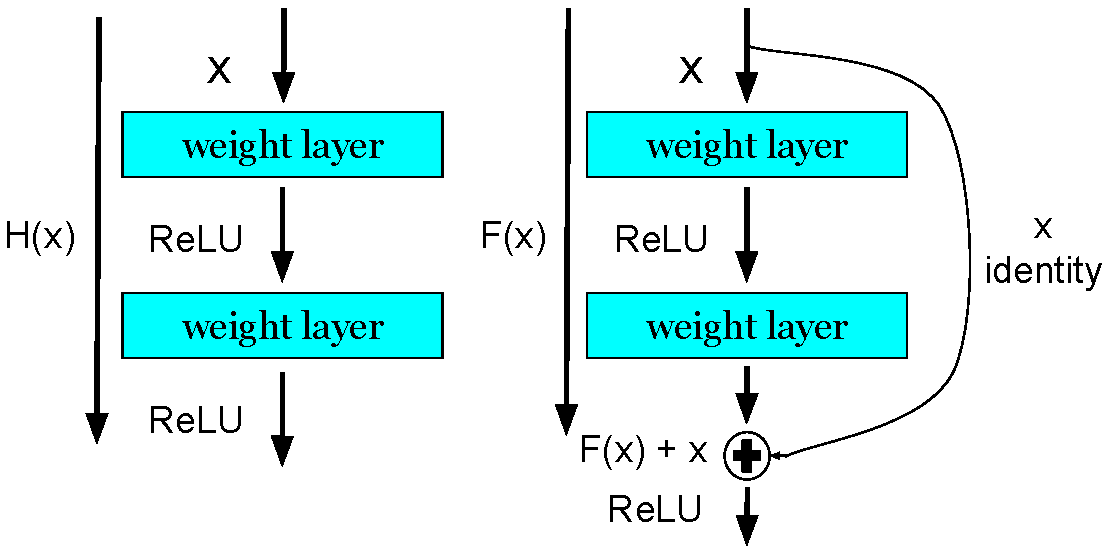
\includegraphics[width=0.8\textwidth]{images/ResNet_1.pdf}
    \end{center}
    \caption{Normal CNN connections vs CNN with residual connections} \label{fig:ResNet_1}
\end{figure}

\subsection{ResNet}
He et al.~\cite{he2016deep} introduced the Residual Block depicted in Figure~\ref{fig:ResNet}(a). However using this residual block, a very deep ResNet arcchitecture gave worse results compared to the shallower 110 layer ResNet. So they refined the residual block and proposed a new version depicted on Figure~\ref{fig:ResNet}(b). With experiments they trained a very deep 1001 layer ResNet that achieved better results by its shallower counterparts.

\begin{figure}[]
    \begin{center}
    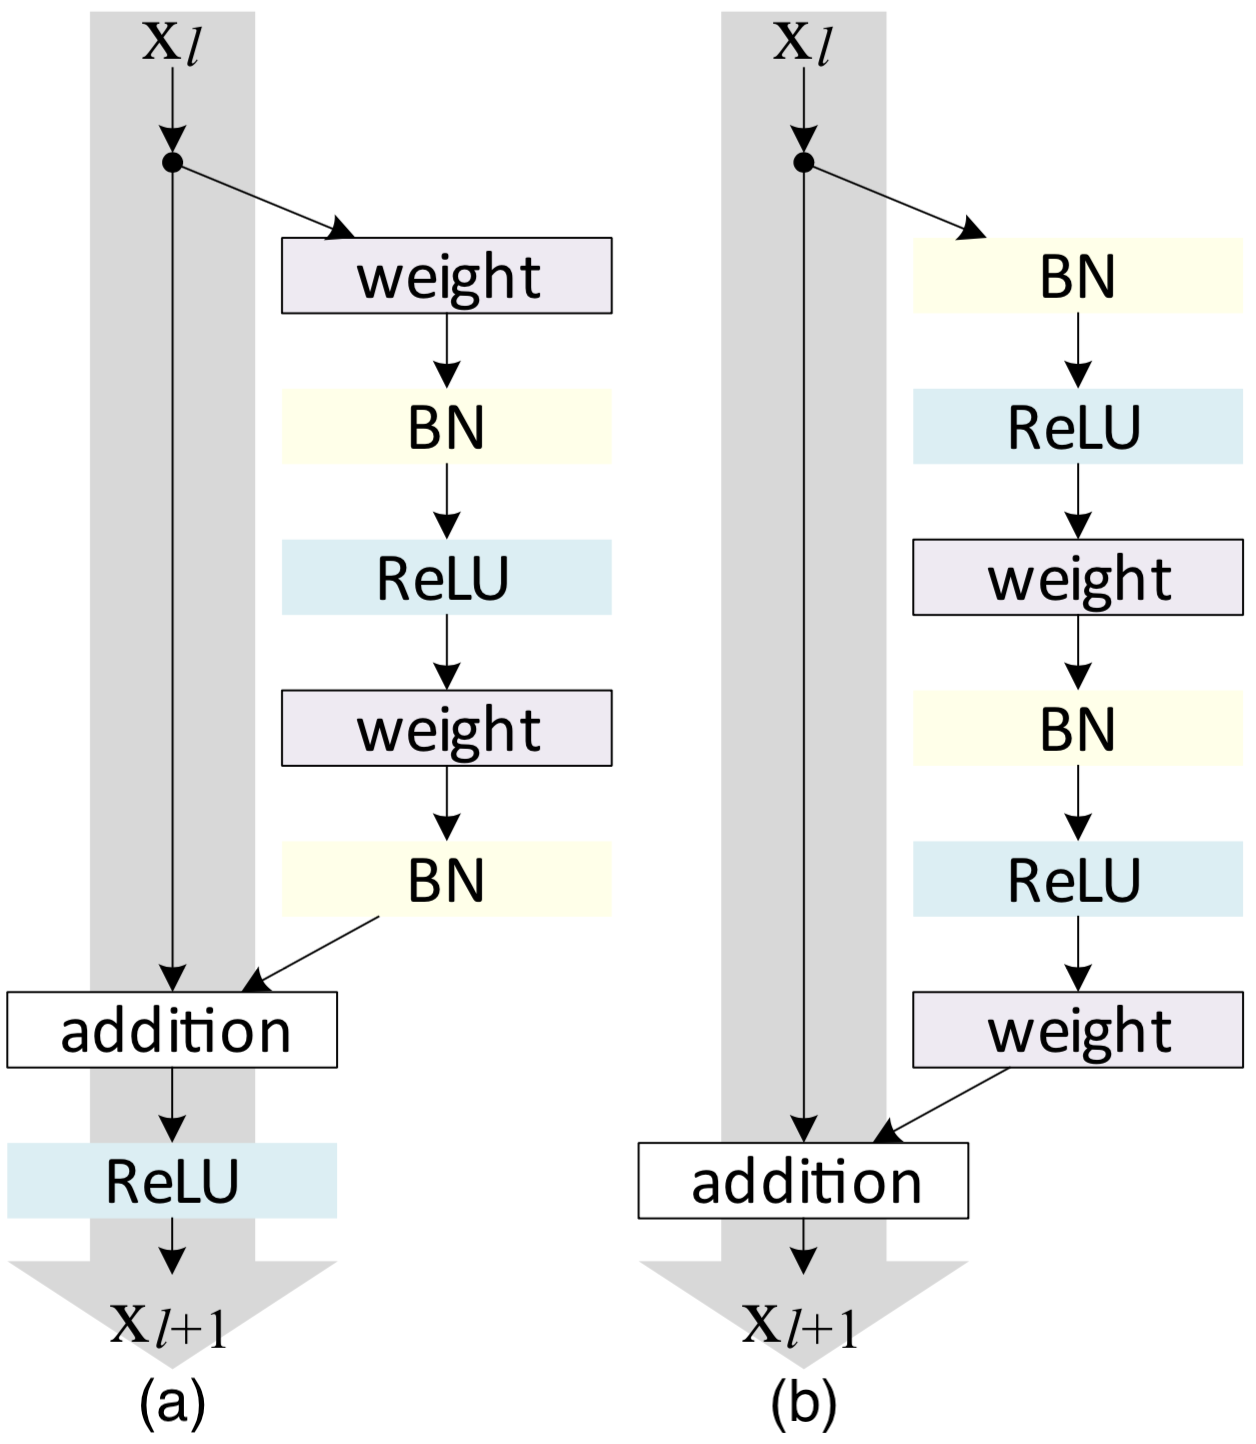
\includegraphics[width=0.6\textwidth]{images/ResNet.png}
    \end{center}
    \caption{(a) original Residual Unit, (b) enhanced Residual Unit. Extracted from~\cite{he2016identity}}\label{fig:ResNet}
\end{figure}

\subsection{DenseNet}
Huang et al.~\cite{huang2017densely} proposed a novel architecture called DenseNet that exploits the effects of shortcut connections. In this architecture all layers are connected to each other. Every layer receives as input the feature maps from all previous layers and sends its output to all subsequent layers. Figure~\ref{fig:DenseNet} gives an example of the network. The authors claim that this architecture except from solving the vanishing gradient problem, it encourages feature re-use, and reduces the number of parameters. However, DenseNets can require a significant amount of GPU memory despite the fact that they have less parameters. DenseNets have much more connections than ResNets, and since Back-propagation requires all layers' output to be in memory, that is the main reason for memory bottlenecks. 

\begin{figure}[]
    \begin{center}
    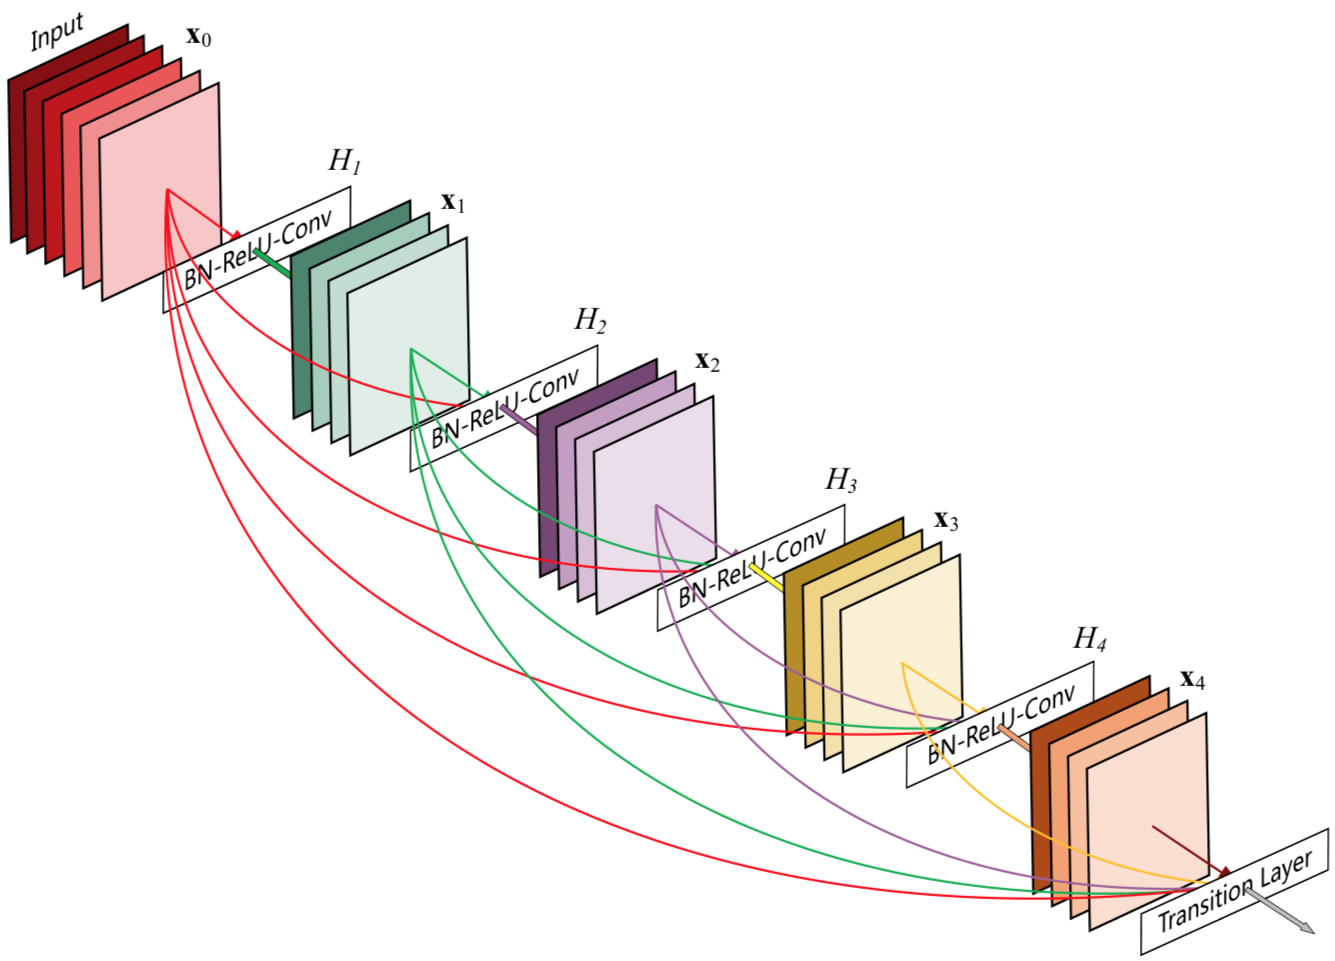
\includegraphics[width=0.6\textwidth]{images/DenseNet.png}
    \end{center}
    \caption{A 5-layer dense block with a growth rate of $k = 4$. Each layer takes as input the feature maps from all previous layers. Extracted from~\cite{huang2017densely}}\label{fig:DenseNet}
\end{figure}

\subsection{Wide ResNet}
Zagoruyko and Komodakis~\cite{zagoruyko2016wide} to tackle the computational and memory contraints of the DenseNet network, instead of increasing the  depth (number of layers) of the network, they experimented by increasing the width (number of neurons per layer or for convolutional layers the number of feature maps per layer) and also using dropout to regularize the wider networks. So a Wide ResNet is just a ResNet with more feature maps in its convolutional layers. They experimented with architectures of different depth and width with the same number of parameters and showed that the wider version performs better on CIFAR-10, CIFAR-100~\cite{krizhevsky2009learning}, and SVHN~\cite{netzer2011reading}. As mentioned in their paper, thin and deep residual networks with small kernels are against the nature of GPU computations because of the sequential structure, as opposed to wide networks that are many times more efficient than the deep and thin network that achieves the same performance. 

%\afterpage{\blankpage}